\documentclass[aspectratio=169]{beamer}
\usepackage{bookmark}
\usepackage{lifa}
\usepackage[style=ieee]{biblatex}
\setbeamertemplate{bibliography item}{\insertbiblabel}
\addbibresource{bibliography.bib}

\title{Adesão Celular}
\subtitle{A Base da Organização Tecidual}
\author{Gustavo O. Rosa}
\institute{Laboratório de Inovação em Física Aplicada}
% \date{\today}

\begin{document}
%% Página de título
%% Remova '[plain]' se precisar de um rodapé
\begin{frame}[plain]
    \titlepage
\end{frame}


% %% Página de Sumário
% {
% \begin{frame}
%     \frametitle{Sumário}
%     \tableofcontents
% \end{frame}
% }


\section{Introdução Biológica}

\begin{frame}{Importância da Ligação Celular}
    \begin{itemize}
        \item \textbf{Desenvolvimento de Órgãos e Manutenção Tecidual}: 
        Garante a coesão e integridade dos tecidos, formando a estrutura complexa dos organismos 
        multicelulares
        \item \textbf{Migração e Sinalização Celular}: Permite que as células se movam de forma
        coordenada e respondam a sinais do seu microambiente, crucial em processos como o 
        desenvolvimento embrionário e a cicatrização de feridas
        \item \textbf{Resposta Imune e Inflamação}: Essencial para a localização e movimentação de 
        células imunes para locais de infecção ou dano
    \end{itemize}
\end{frame}

\begin{frame}{Tipos de Ligação}
    As ligações devem ser não-covalentes para manter a dinâmica das células, existem diversas moléculas responsáveis, entre elas:
    \begin{itemize}
        \item \textbf{Caderinas}
        \item Grupo Ig
        \item \textbf{Integrinas}
        \item Selectinas 
        \item Mucinas
    \end{itemize}
    Essas ligações tem dois grandes grupos: \textbf{célula-célula} e \textbf{célula-matriz}
\end{frame}

\begin{frame}{Tipos de Ligação}
    \begin{figure}\label{fig:ligacao_geral}
        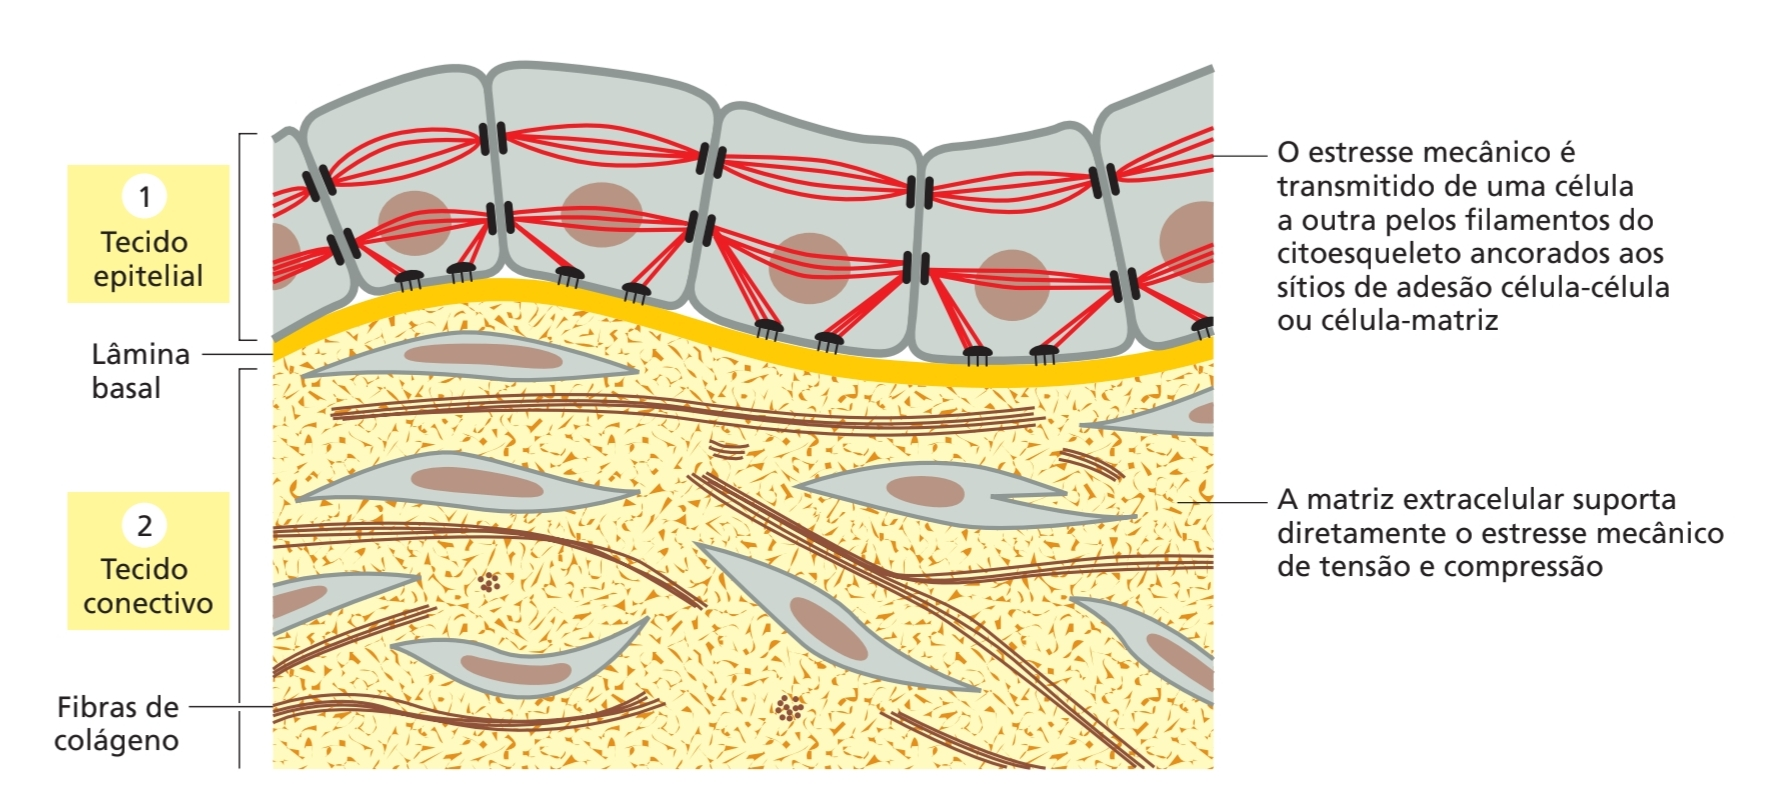
\includegraphics[width=0.9\textwidth]{img/bio/tipos_ligação.jpg}
        \caption{Imagem representativa dos tipos de ligação célula-célula e célula-matriz}
    \end{figure}
\end{frame}


\begin{frame}{Caderinas}
    \begin{columns}[c, onlytextwidth]
        \column{0.5\textwidth}
            \begin{itemize}
               \item As caderinas são responsáveis pelas ligações \textbf{célula-célula}
               \item A sua função é estritamente dependente de \textbf{íons cálcio}
               \item Processo dinâmico de ligação e dissociação
            \end{itemize}
        
        \column{0.5\textwidth}
            \begin{figure}\label{fig:caderinas}
                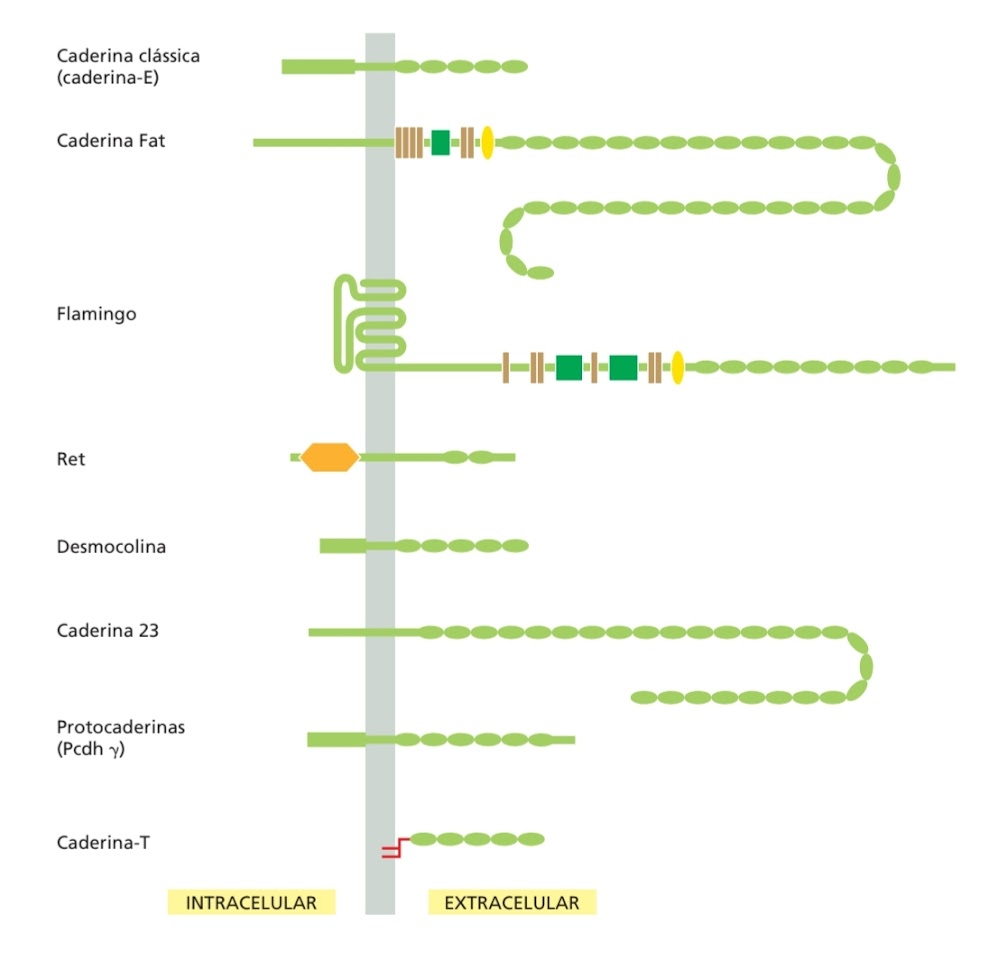
\includegraphics[width=0.9\textwidth]{img/bio/caderinas.jpg}
                \caption{Diferentes tipos de caderinas}
            \end{figure}
    \end{columns}
\end{frame}

\begin{frame}{Caderinas}
    \begin{figure}
        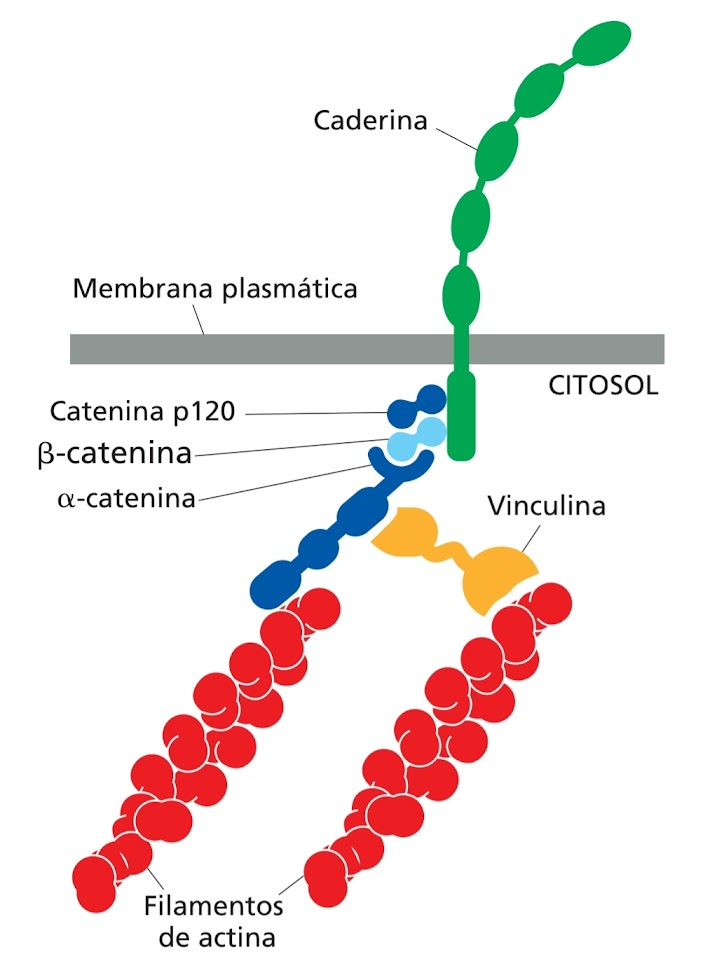
\includegraphics[width=0.32\textwidth]{img/bio/close_caderina.jpg}
        \caption{Visão geral da caderina}
    \end{figure}
\end{frame}

\begin{frame}{Outras ligações}
    \begin{columns}[t, onlytextwidth]
        \column{0.5 \textwidth}
            \begin{itemize}
                \item A \textbf{superfamília IG} liga em proteínas, como fibronectina, lamina e 
                colágeno e se ligam de forma homofílica ou heterofílica
                \item \textbf{Selectinas} se ligam com as \textbf{mucinas} em regiões com carboidratos
                e são responsáveis pela ligação incial de leucócitos em células endoteliais 
            \end{itemize}    

        \column{0.5\textwidth}
            \begin{figure}\label{fig:hetero_homo}
                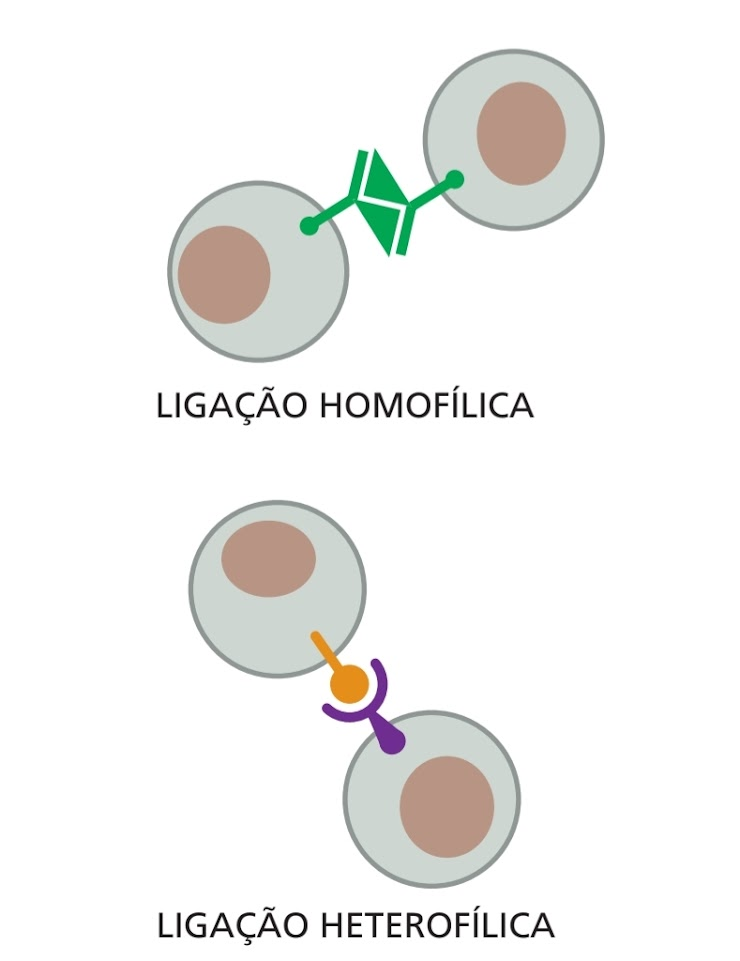
\includegraphics[width=0.6\textwidth]{img/bio/hetero_homo_bonds.jpg}
                \caption{Ligações heterofílica e homofílica}
            \end{figure}
    \end{columns}
\end{frame}

\begin{frame}{Ligações Célula-Célula}
    \begin{figure}
        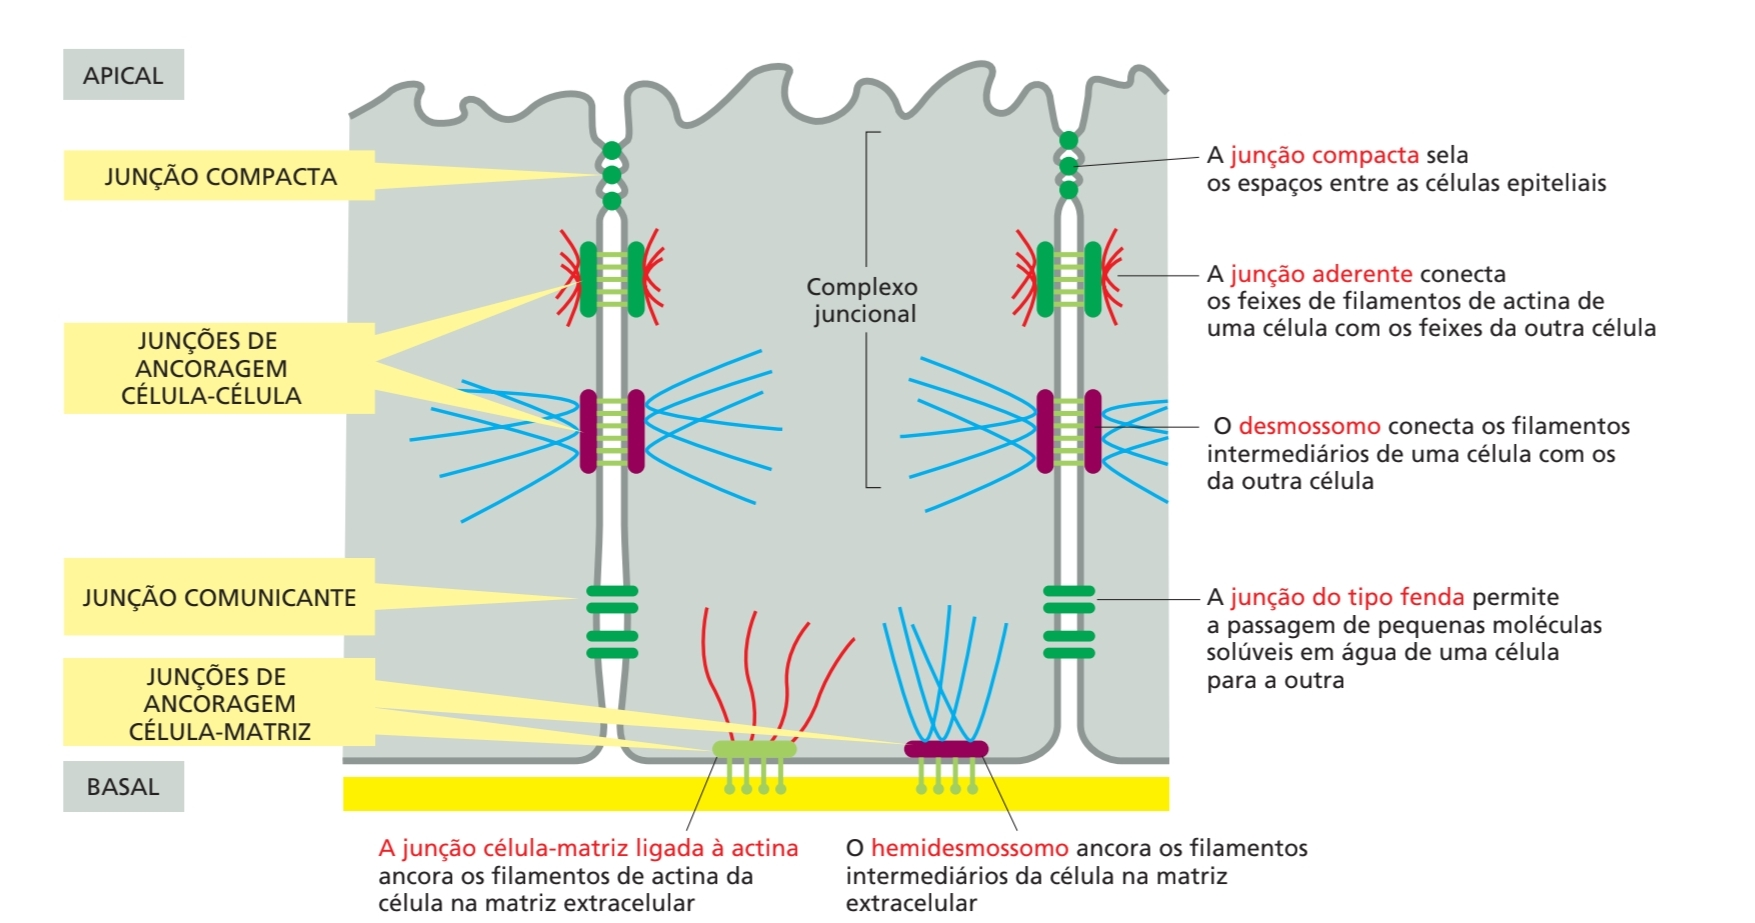
\includegraphics[width=0.8\textwidth]{img/bio/celula_celula.jpg}
        \caption{Tipos de ligação célula-célula}
    \end{figure}
\end{frame}

\section{Efeito de Forças nas Ligações}
\begin{frame}
    \begin{figure}
        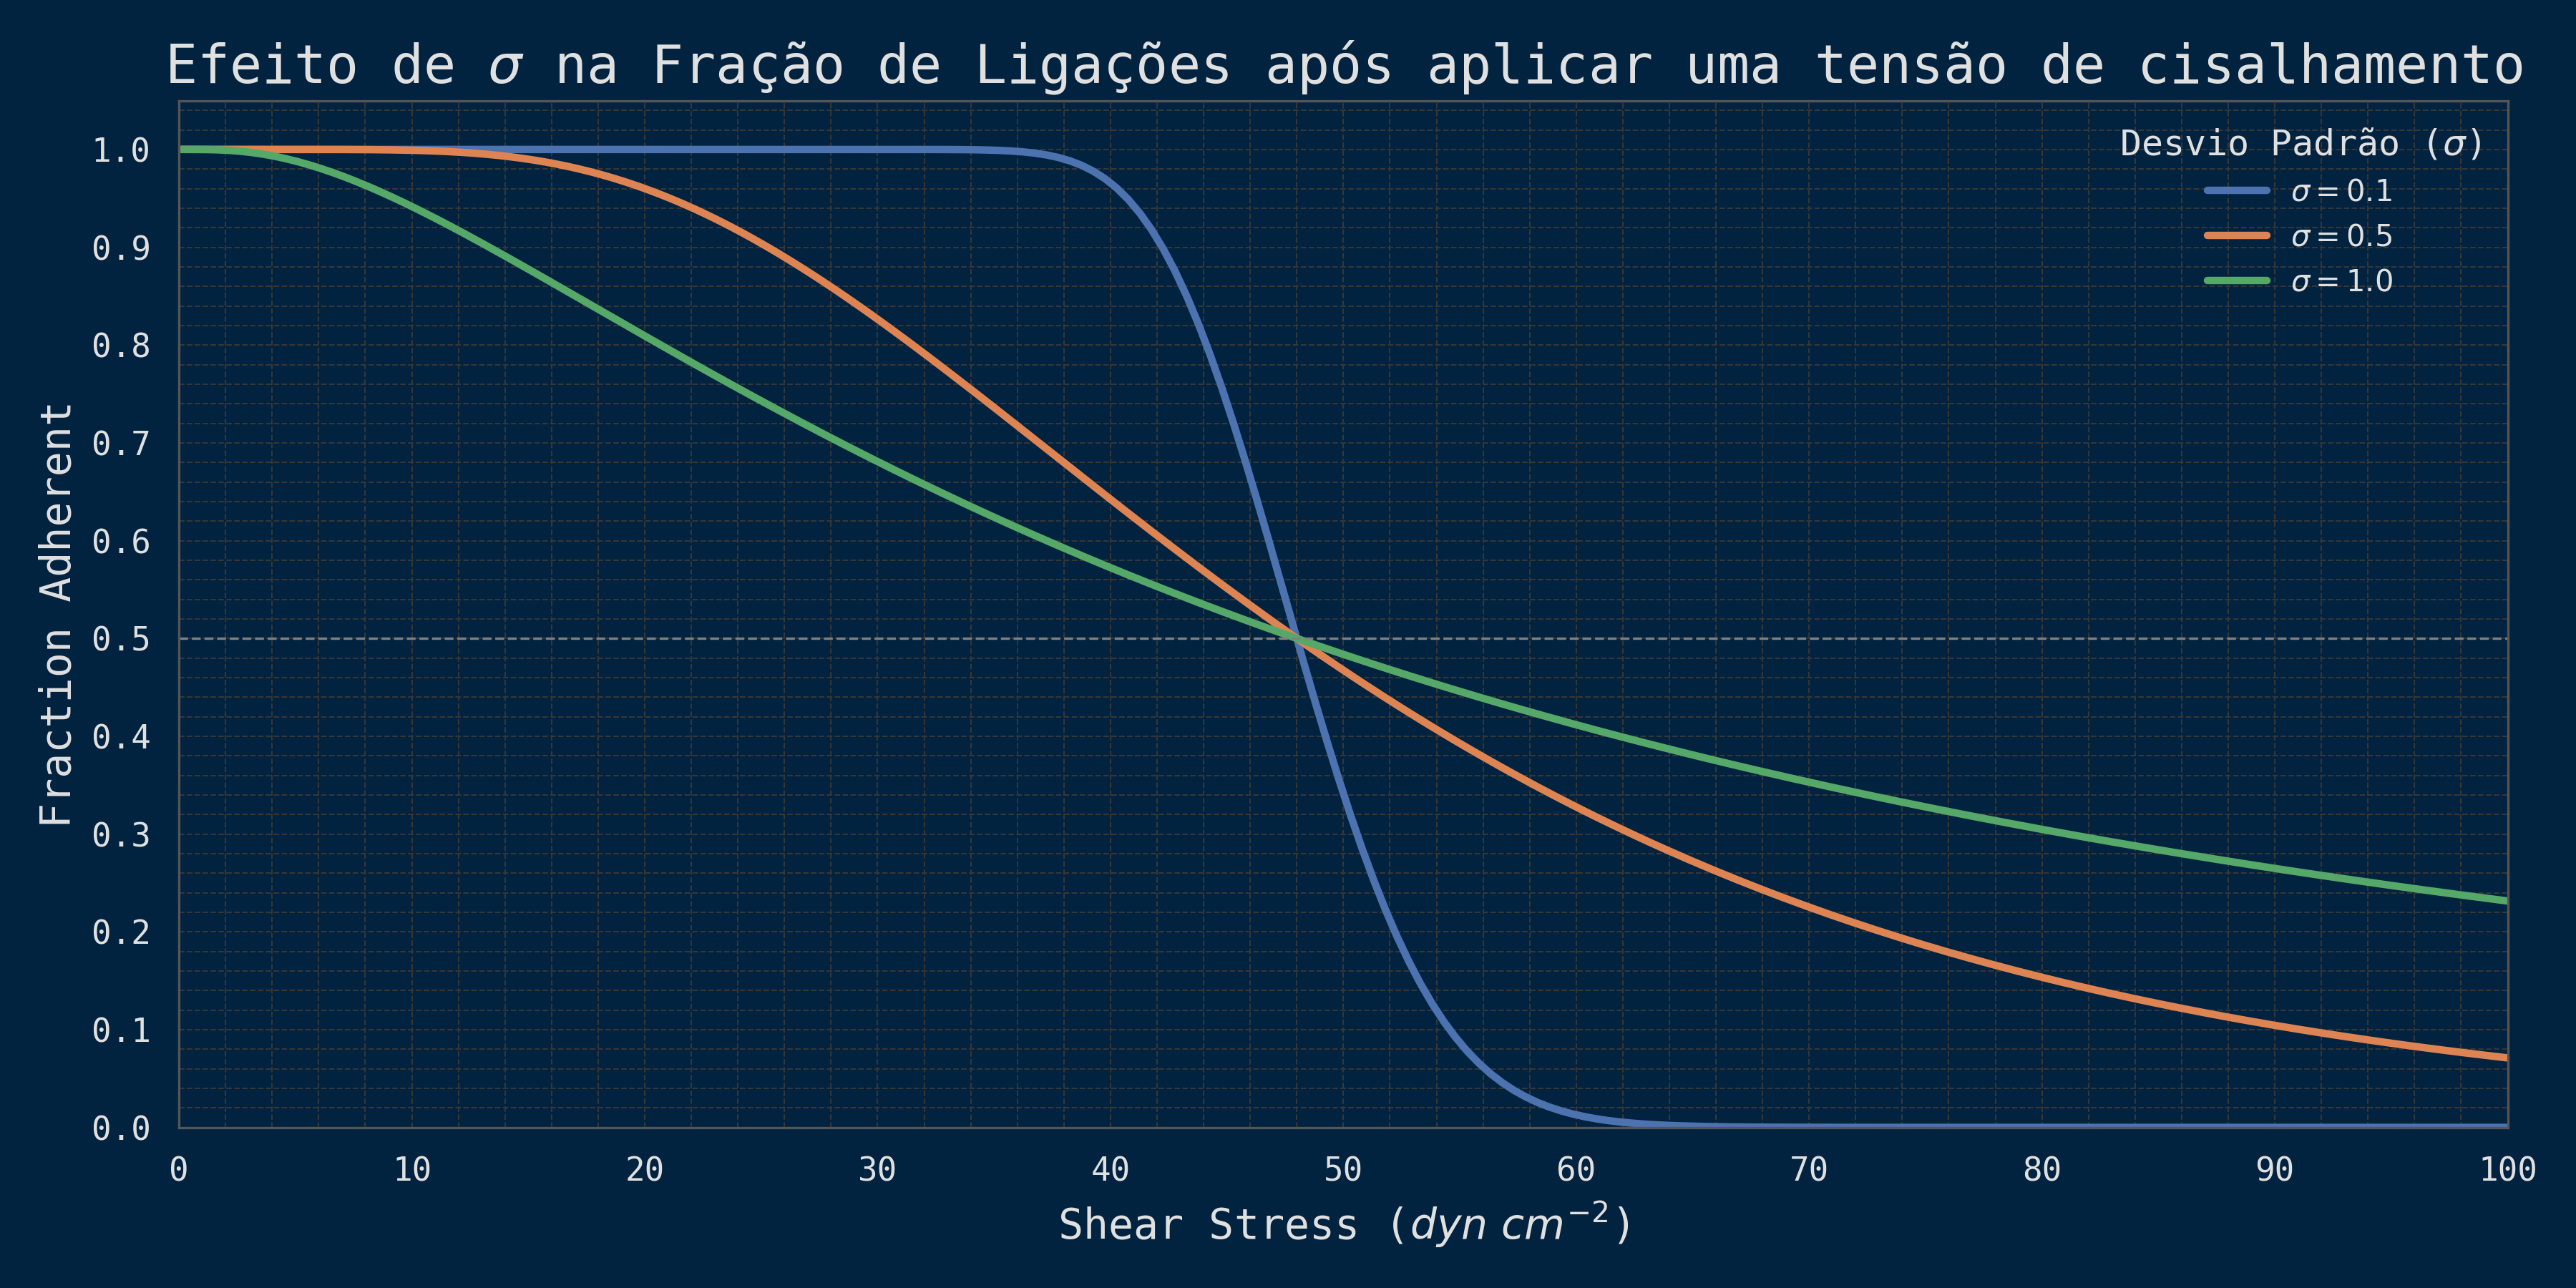
\includegraphics[width=0.9\textwidth]{img/sigma_cisalhamento.png}
    \end{figure}
\end{frame}

\end{document}
